\documentclass{beamer}

% Setup appearance:

\usetheme{Darmstadt}
\usefonttheme[onlylarge]{structurebold}
\setbeamerfont*{frametitle}{size=\normalsize,series=\bfseries}
\setbeamertemplate{navigation symbols}{}


% Standard packages

\usepackage[brazil]{babel}
\usepackage[latin1]{inputenc}
\usepackage{times}
\usepackage[T1]{fontenc}
\usepackage{amsmath}% http://ctan.org/pkg/amsmath
%\usepackage[table]{xcolor}
\usepackage{multicol}
\usepackage{textcomp} 


\begin{document}

\begin{frame}
  \titlepage
\end{frame}

\begin{frame}
  \tableofcontents
\end{frame}

\section{Weka}
\begin{frame}
	\begin{itemize}
		\item Programa que possui uma cole��o de algoritmos de aprendizagem de m�quina para usar em tarefas de minera��o de dados
		\item Desenvolvido pelo Machine Learning Group da Universidade de Waikato 
		\item O Weka permite que se trabalhe sobre o dataset e traz ferramentas para: pr�-processamento, classifica��o, regress�o, clusteriza��o, regras de associa��o e visualiza��o 
		\item Todos os nossos resultados foram feitos com o apoio do Weka
	\end{itemize}
\end{frame}

\section{Floresta Rand�mica}
\subsection{Random Forest}
\begin{frame}{Floresta Rand�mica (Random Forest)}
		\begin{itemize}
			\item Tudo come�ou em 1996, com o surgimento do meta-algoritmo de Bagging (Bootstrap Aggregating), por Leo Breiman 
			\item Bootstrap ajuda a reduzir vari�ncia e overfitting
				\begin{itemize}
					\item Escolhe aleatoriamente amostras, Di, de um conjunto de treino, D
					\item Esse conjunto de treino D tem reposi��o (ou seja, uma amostra pode ser escolhida mais de uma vez)
					\item Tamanho do conjunto de treino: n
					\item Tamanho do conjunto de amostra: n'
					\item Geralmente n' < n
					\item Quando n' for praticamente n, nota-se uma chance de 63\% de aparecer amostras n�o repetidas. Daqui que surgiu o nome de Bootstrap
				\end{itemize}
		\end{itemize}		
	\end{frame}

\subsection{Random Forest}
\begin{frame}{Floresta Rand�mica (Random Forest)}
	\begin{itemize}
		\item Em 2001, Breiman lan�ou o Random Forest
		\item � um m�todo usado para classifica��o (e regress�o)
		\item O m�todo faz a constru��o de v�rias �rvores de decis�o, com a diferen�a de que n�o usa pruning (poda)
		\item Algoritmo:
			\begin{itemize}
			 	\item Escolhe-se aleatoriamente a amostra (bootstrap) Di dentre D
			 	\item Constr�i a �rvore Ti usando amostra Di
			 	\item Em cada �rvore Ti, escolhe aleatoriamente M vari�veis e encontra a melhor divis�o (split)
			\end{itemize}
		\item No fim, pode-se 
			\begin{itemize}
				\item pegar o voto majorit�rio (classifica��o)
				\item calcular a m�dia dos resultados (regress�o)
			\end{itemize}
	\end{itemize}
\end{frame}

\begin{frame}{Exemplo de Random Forest}
		\begin{figure}[h]
			\centering
			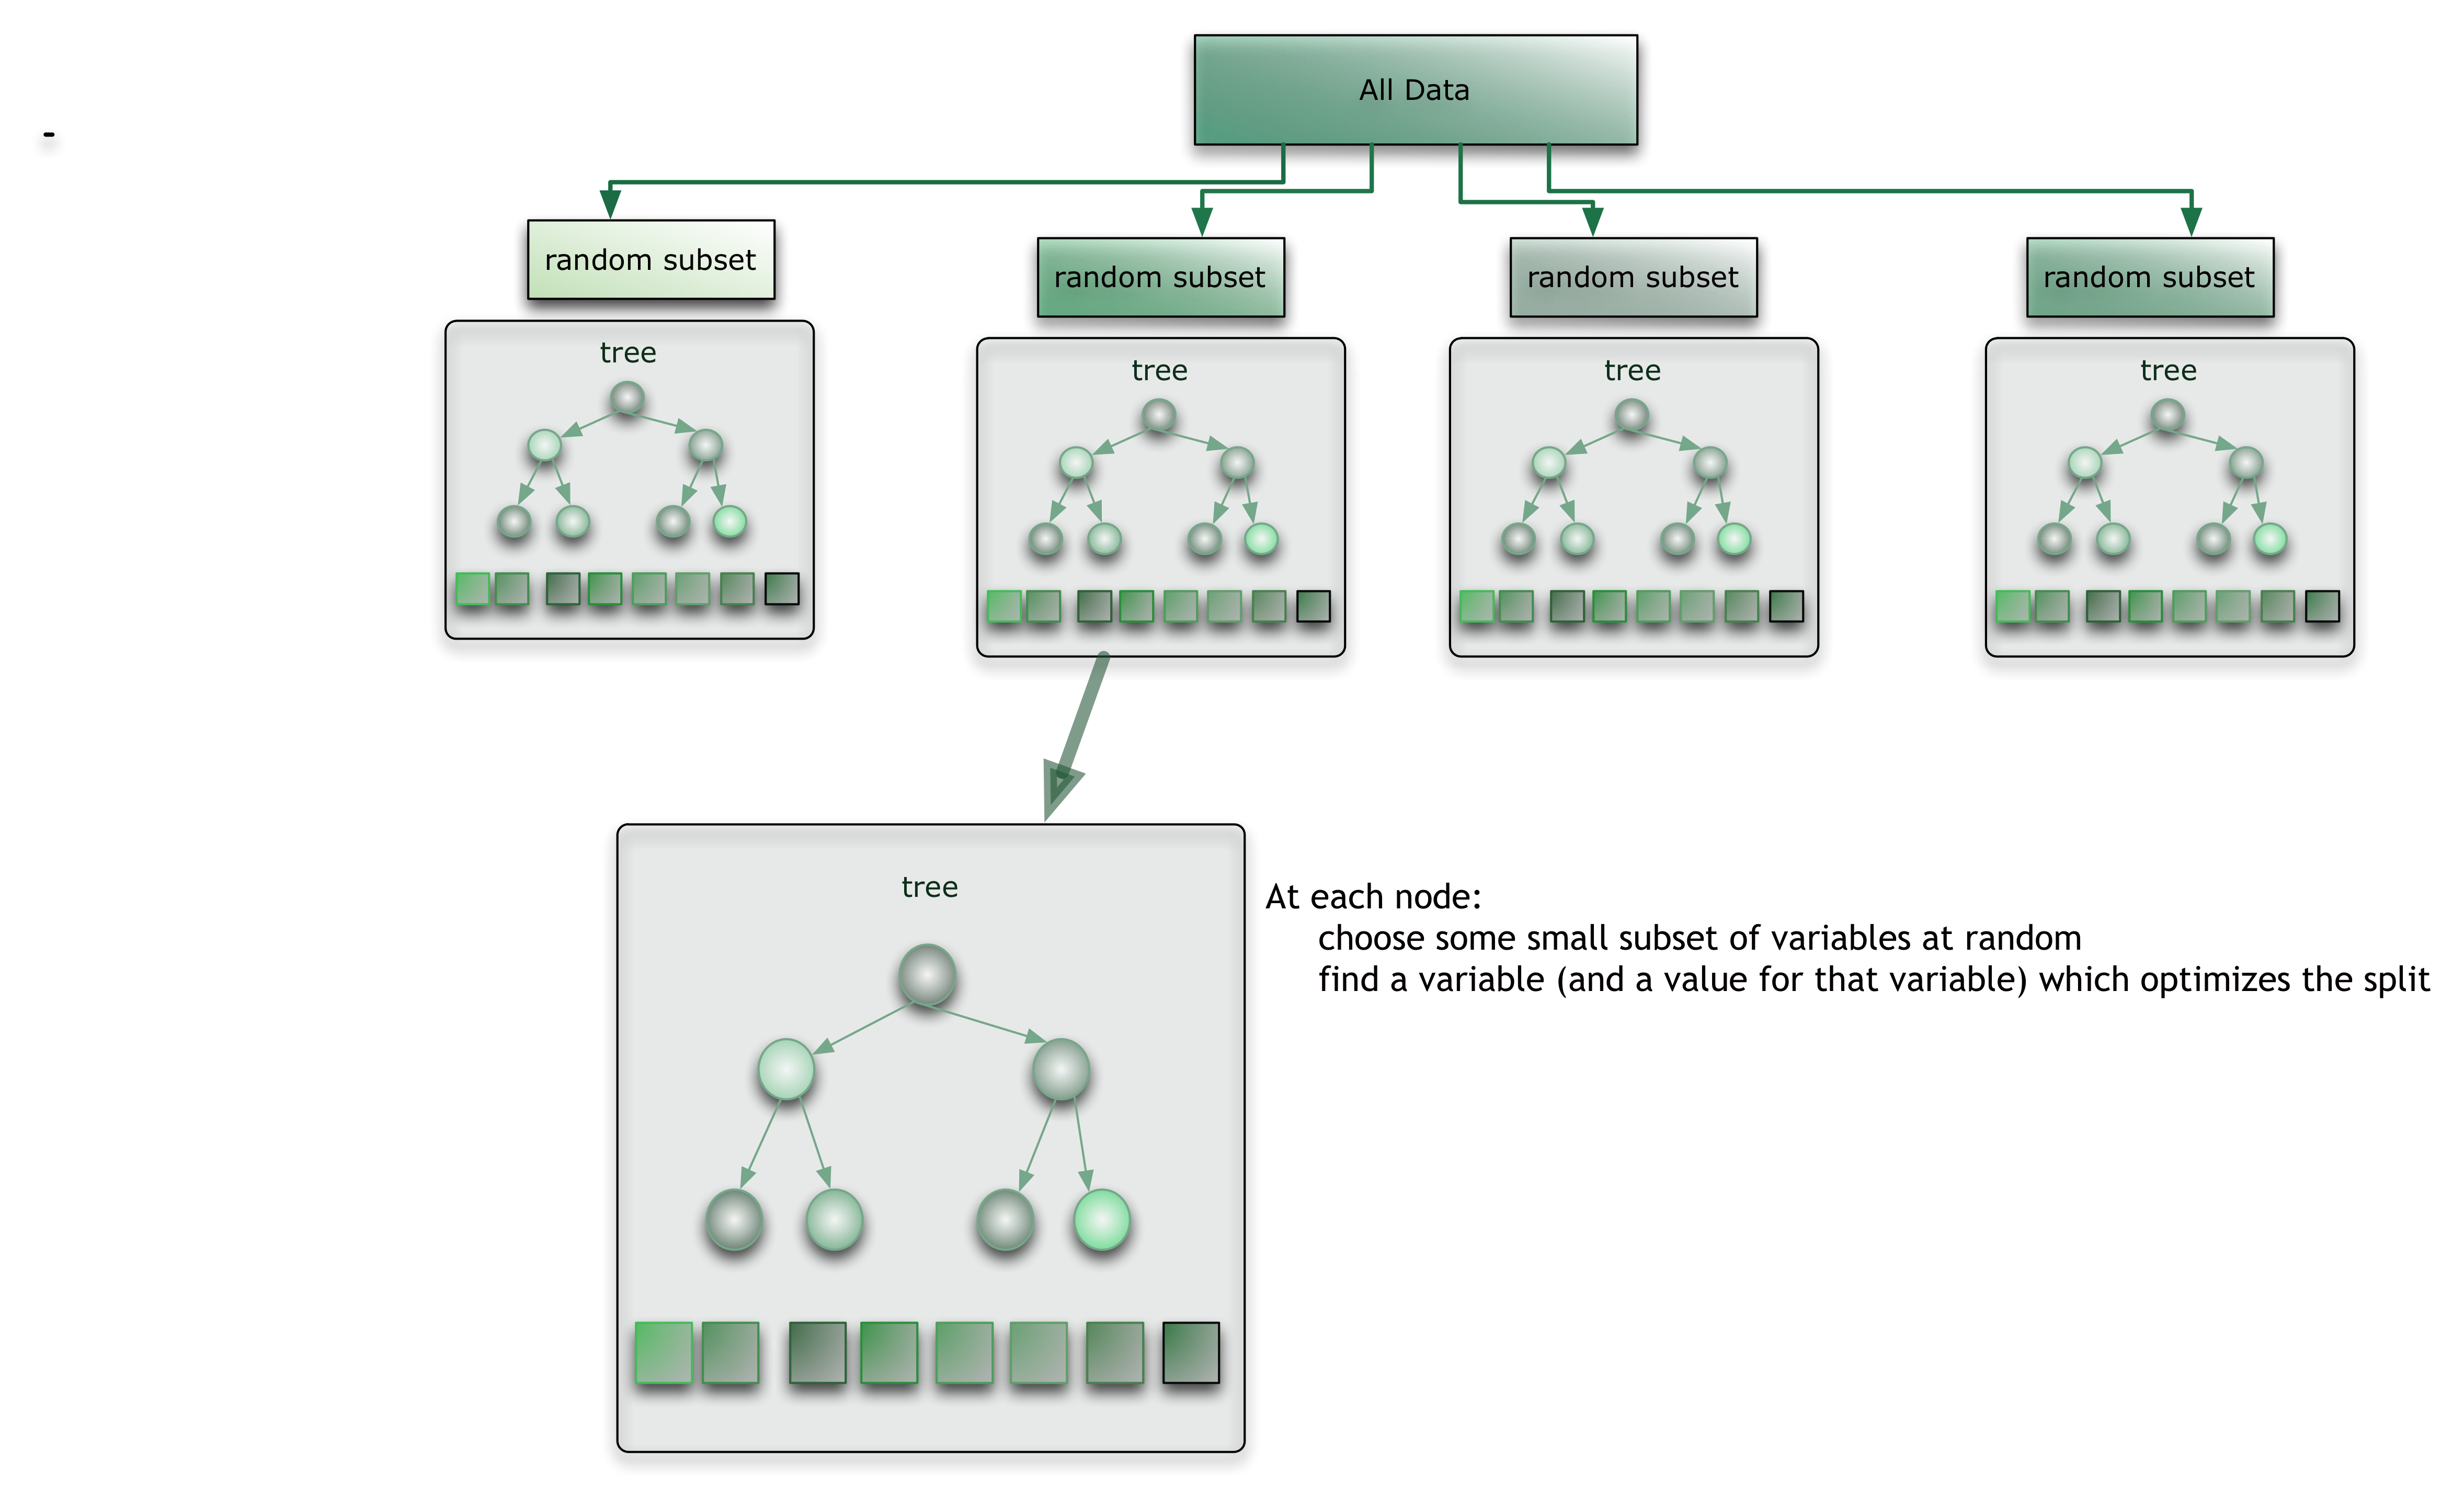
\includegraphics[scale=0.1]{./pictures/RandomForestIago.png}
			%\caption{$ \alpha = 0.8$, N_t = 10, T_max = 2048}
			\label{fig:Random Forest}
		\end{figure}
	\end{frame}
	
\section{Prisma}

\section{Outro Algoritmo}

\section{Compara��oes e Conclus�es}


\end{document}